% =====================================================================
% jcdcg3_slides.tex -- JCDCG^3 2026, Submission 63
% 15 min including Q&A, 1 min changeover -> aim for ~11 min of talk.
%
% The title is the one submitted; the program lists it, so it does not
% change even though the paper has since grown.
%
% Structure: the accepted abstract carries slides 2-7.  Slides 8-9 are
% the additions, and they are placed in that order on purpose.  The
% abstract itself asked whether validity survives every tie-breaking;
% slide 8 answers it for four of the six, and slide 9 is then a warning
% that the answer does not carry to the uniform case -- a corollary of
% slide 8 rather than a separate topic.
%
% Theme is deliberately plain; pick a real one later.
% =====================================================================
\documentclass[aspectratio=169,11pt]{beamer}

\usetheme{default}
\usecolortheme{dove}
\setbeamertemplate{navigation symbols}{}
\setbeamertemplate{footline}[frame number]
\setbeamertemplate{itemize items}[circle]
\setbeamerfont{frametitle}{size=\large,series=\bfseries}
\setbeamercolor{alerted text}{fg=red!70!black}

\usepackage{booktabs}
\usepackage{graphicx}
\usepackage{amsmath,amssymb}

\newcommand{\RR}{\mathbb{R}}

\title{Face-Rotation BFS Nets of the\\Six Regular Convex 4-Polytopes}
\author{Takashi Yoshino}
\institute{Toyo University, Japan\\\texttt{tyoshino@toyo.jp}}
\date{JCDCG\textsuperscript{3} 2026}

\begin{document}

% ---------------------------------------------------------------- 1
\begin{frame}
  \titlepage
\end{frame}

% ---------------------------------------------------------------- 2
\begin{frame}{Unfolding a 4-polytope}
  \begin{columns}[T]
    \begin{column}{0.58\textwidth}
      A \alert{net} of a convex polytope: cut it open and lay the
      facets out flat, without overlap.
      \medskip

      In 3D this is D\"urer's problem, still open.
      \medskip

      In 4D the facets are \alert{3-dimensional cells} and the net
      lives in $\RR^3$.
      \begin{itemize}
        \item Turney (1984): all 261 nets of the 8-cell
        \item Devadoss--Harvey (2023): \emph{every} spanning tree works
          for the 5-, 8-, 16-cell
      \end{itemize}
      \medskip

      \alert{Left open: 24-cell, 120-cell, 600-cell.}
    \end{column}
    \begin{column}{0.4\textwidth}
      \centering
      \includegraphics[width=\textwidth]{face_rotation_net_5cell.png}\\
      {\scriptsize A net of the 5-cell}
    \end{column}
  \end{columns}
\end{frame}

% ---------------------------------------------------------------- 3
\begin{frame}{Face-rotation BFS}
  Fix a \alert{root cell} $r$. Three steps.
  \medskip

  \begin{enumerate}
    \item[\textbf{1}] \textbf{Face-up.} Rotate in $SO(4)$ so the
      centroid of $r$ sits on the $+w$ axis.
    \item[\textbf{2}] \textbf{BFS.} Take a breadth-first spanning tree
      of the cell-adjacency graph from $r$. For each tree edge
      (parent $p$, child $c$), rotate $c$ about the shared polygon
      until it lands in $p$'s hyperplane.
    \item[\textbf{3}] \textbf{Project.} All cells now share one
      $w$-coordinate (spread $<4\times10^{-13}$). Drop $w$.
  \end{enumerate}
  \medskip

  The result is a net iff no two cells share interior volume.
\end{frame}

% ---------------------------------------------------------------- 4
\begin{frame}{The validity test, and a trap}
  A net is valid if for every pair of cells not joined by a tree edge,
  \[
    \mathrm{Vol}_3\bigl(\mathrm{conv}(c_i)\cap\mathrm{conv}(c_j)\bigr)
    \;\le\; 10^{-8}.
  \]
  \medskip

  \begin{alertblock}{Boundary contact is not overlap}
    Testing with closed-region membership instead counts a shared face,
    edge or vertex as an intersection.
    That is common for pointed cells, and it wrongly reports
    \[
      \text{16-cell } 0/16, \quad
      \text{24-cell } 0/24, \quad
      \text{600-cell } 0/600 .
    \]
    Measuring \emph{volume} ignores contact of measure zero.
  \end{alertblock}
\end{frame}

% ---------------------------------------------------------------- 5
\begin{frame}{Main result}
  \begin{block}{Theorem}
    For every regular convex 4-polytope and \alert{every} root cell,
    the face-rotation BFS net is valid.
  \end{block}
  \medskip

  \centering
  \includegraphics[width=0.62\textwidth]{260612AllFaceRotation.pdf}

  \raggedright\smallskip
  {\small $5+8+16+24+120+600=773$ roots, all verified.
  New beyond Devadoss--Harvey: the 24-, 120- and 600-cell.}
\end{frame}

% ---------------------------------------------------------------- 6
\begin{frame}{Contrast: the apple-peel algorithm}
  A different family of spanning trees --- a greedy spiral/zonal
  ordering (Yoshino--Chaidee).
  \medskip

  \centering
  \begin{tabular}{lccc}
    \toprule
    & BFS & \multicolumn{2}{c}{apple-peel (RZ)}\\
    \cmidrule(lr){3-4}
    Polytope & valid & orderings & nets\\
    \midrule
    120-cell & all roots & $1440/1440$ & \alert{$0/1440$}\\
    600-cell & all roots & \alert{$0/2400$} & ---\\
    \bottomrule
  \end{tabular}

  \raggedright\bigskip
  The 120-cell has an ordering for every start and \alert{never} a net;
  the 600-cell has no ordering at all.
  \medskip

  \begin{block}{}
    Having a valid \emph{ordering} and having a valid \emph{net} are
    independent properties.
  \end{block}
\end{frame}

% ---------------------------------------------------------------- 7
\begin{frame}{And more: the tie-breaking question}
  The abstract left this open:
  \begin{quote}\small
    ``Whether validity extends to all BFS tie-breakings \dots\ remains
    open.''
  \end{quote}
  \medskip

  BFS layers do not depend on the rule, so a BFS tree is just a choice
  of parent, one layer up, for each cell --- and the trees can be
  counted and enumerated with no rule at all.
  \medskip

  \centering
  \begin{tabular}{lrr}
    \toprule
    & trees per root & checked\\
    \midrule
    5-cell   & $1$          & all\\
    8-cell   & $6$          & all\\
    16-cell  & $20{,}736$   & all\\
    24-cell  & $32{,}768$   & all\\
    \midrule
    120-cell & ${\sim}1.8\times10^{44}$ & 20 random / root\\
    600-cell & ${\sim}1.8\times10^{65}$ & 20 random / root\\
    \bottomrule
  \end{tabular}

  \raggedright\medskip
  \alert{$1{,}132{,}661$ trees, no self-intersection.}
  For the first four the rule is irrelevant --- including the 24-cell,
  one of the open cases.
\end{frame}

% ---------------------------------------------------------------- 8
\begin{frame}{$\triangle$ Warning: this does not extend}
  \begin{columns}[T]
    \begin{column}{0.55\textwidth}
      Beyond the regular case the rule stops being harmless.
      \medskip

      \begin{alertblock}{Grand antiprism, 320 cells}
        \centering
        \begin{tabular}{ll}
          rule A & valid from \alert{all $320$} roots\\
          rule B & valid from \alert{no} root\\
        \end{tabular}
      \end{alertblock}
      \medskip

      Same polytope, same roots, same family of BFS trees.
      Only the choice of parent differs.
      \medskip

      Among the 64 convex uniform 4-polytopes this is not isolated:
      others swing from $1.8\%$ to $99.8\%$ of their roots.
    \end{column}
    \begin{column}{0.42\textwidth}
      \centering
      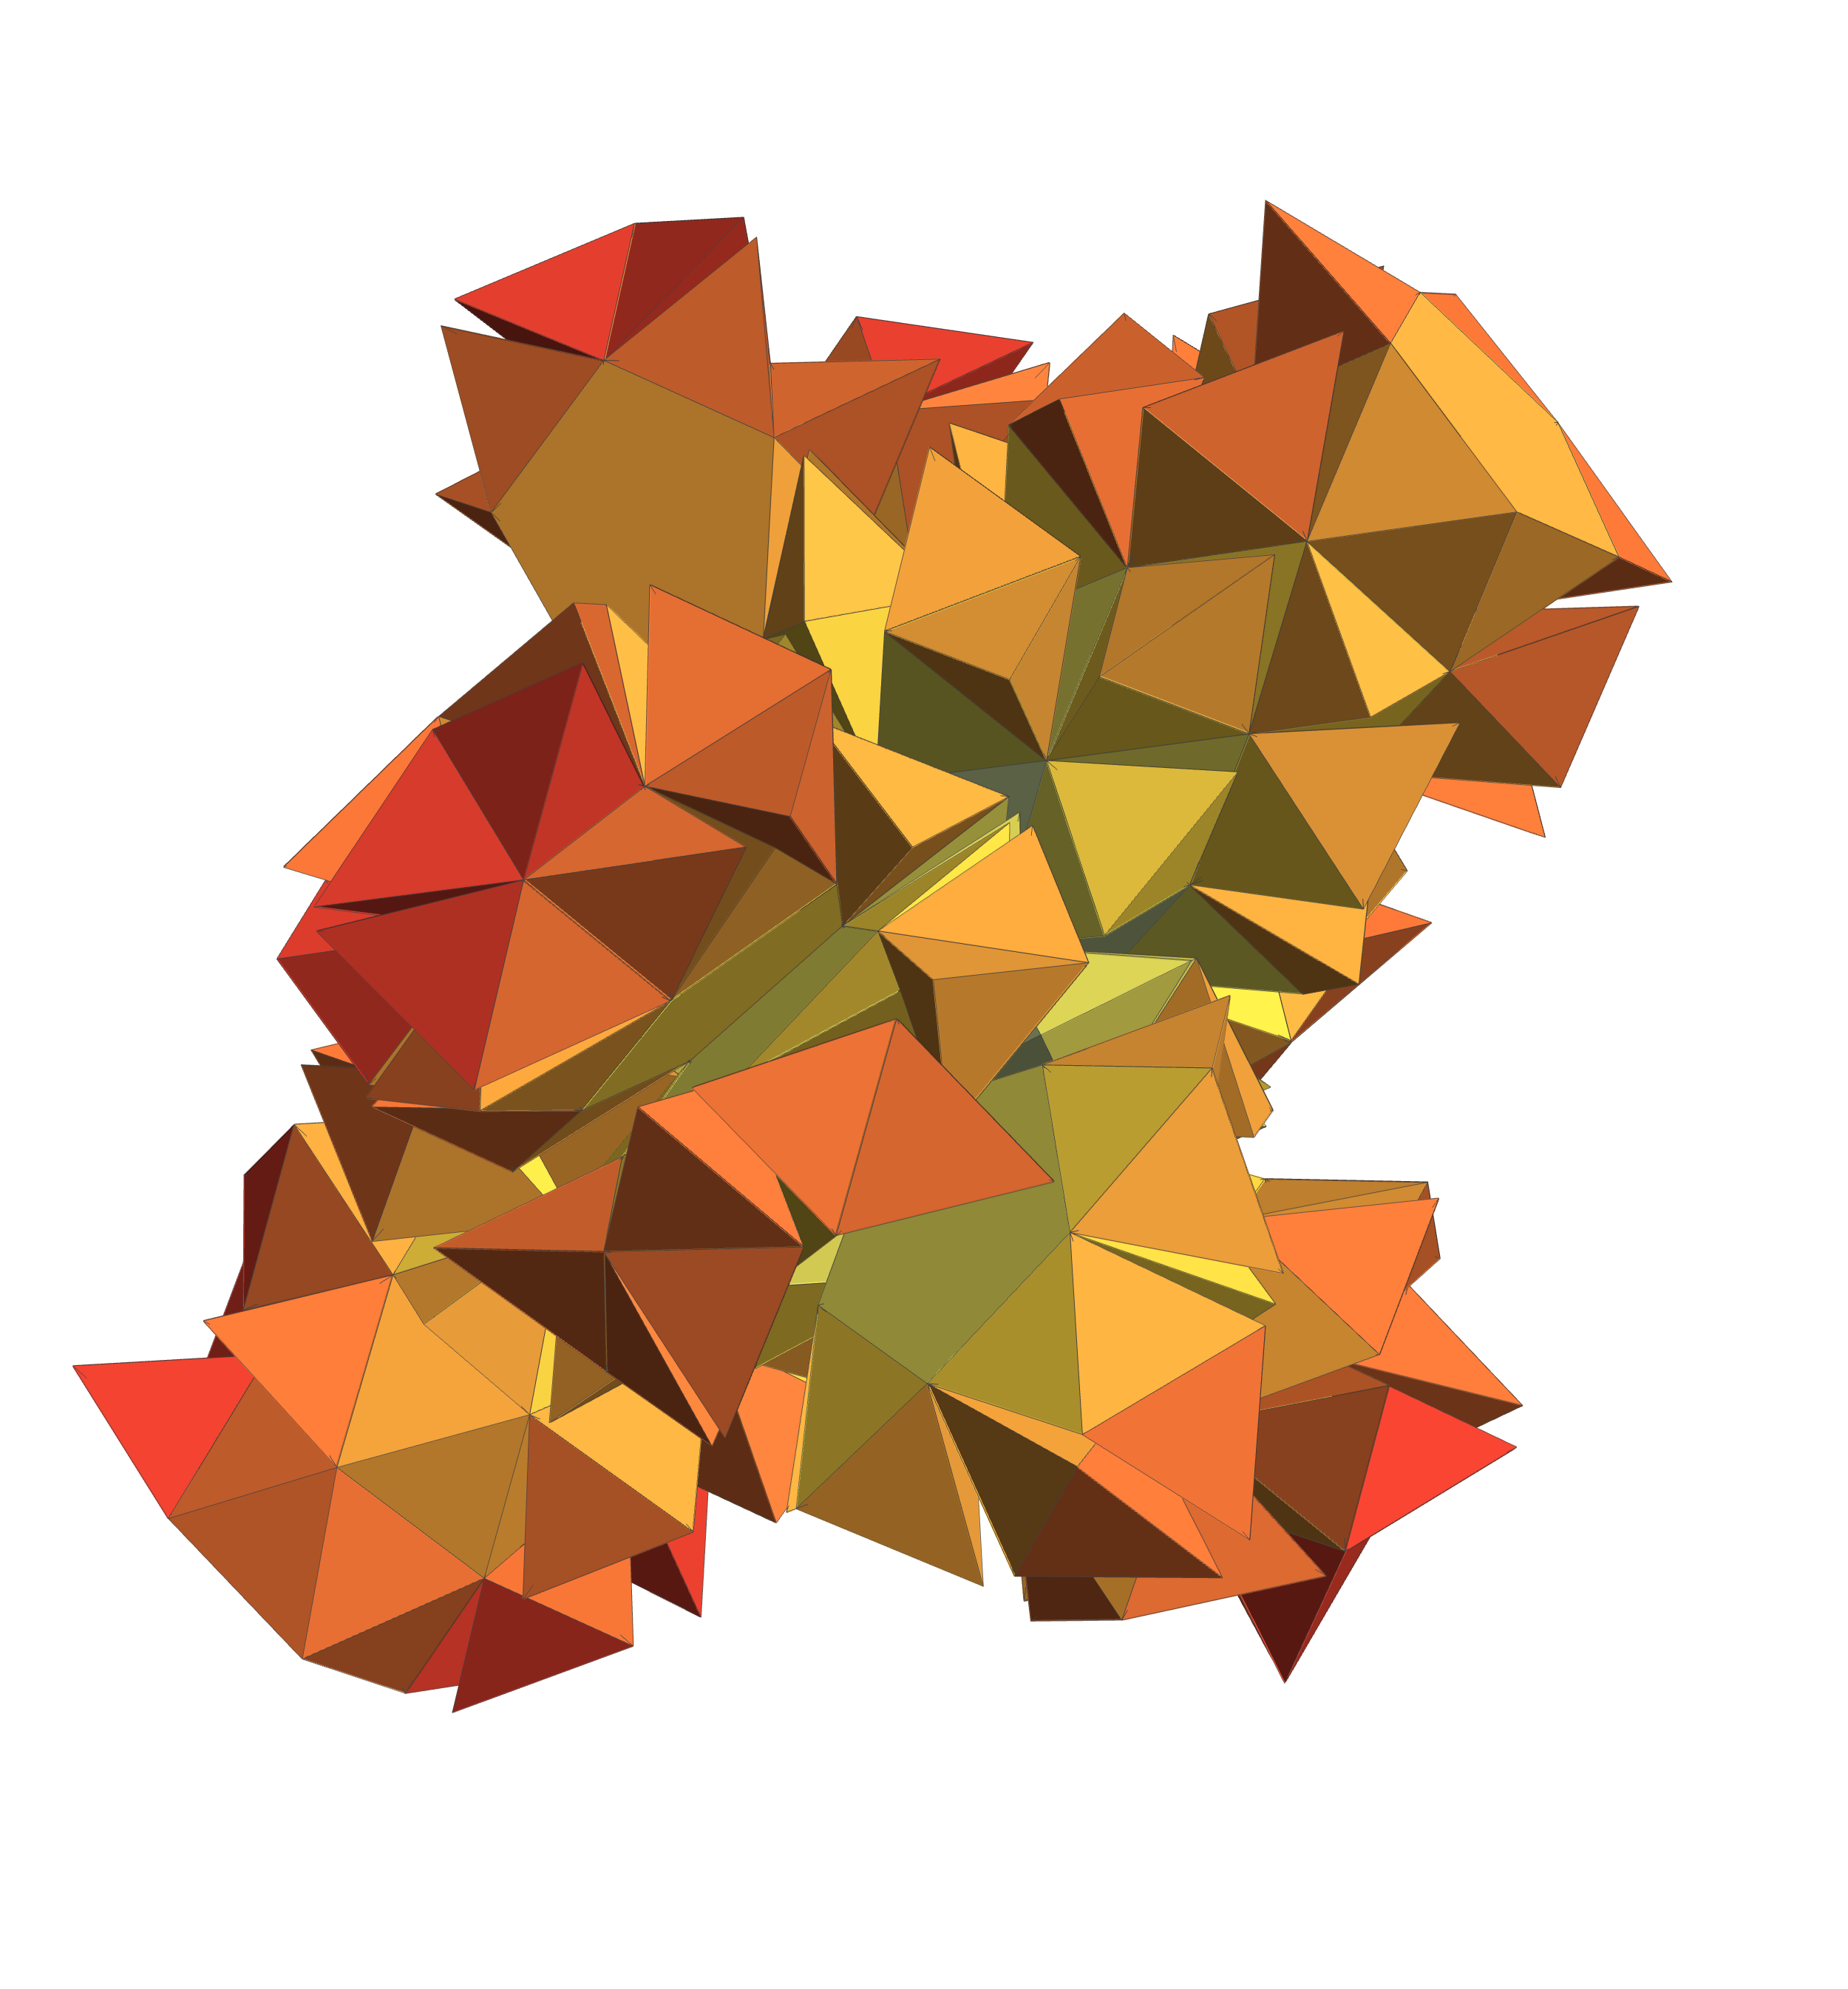
\includegraphics[width=\textwidth]{talk_gap.png}\\
      {\scriptsize Grand antiprism, one valid net}
    \end{column}
  \end{columns}
  \medskip

  \centering
  \textbf{What regularity buys is not that some tree works,
  but that the choice does not matter.}
\end{frame}

% ---------------------------------------------------------------- 9
\begin{frame}{Open problems}
  \begin{itemize}
    \item Why? A proof that does not enumerate.
    \item From BFS trees to \alert{all} spanning trees --- still open
      for the 24-, 120- and 600-cell.
    \item For the 120- and 600-cell even the BFS family is open:
      $10^{44}$ and $10^{65}$ trees per root put enumeration out of
      reach, so an argument would have to be structural.
    \item What separates the uniform polytopes that are insensitive to
      the rule from those that are not?
  \end{itemize}
  \vfill
  \centering
  \small Code, data and nets:
  \texttt{github.com/takashi-randomwalker/apple-peel-4d}
\end{frame}

% ================================================================
\appendix

% ---------------------------------------------------------------- B1
\begin{frame}{Backup: ``BFS tree'' is bigger than what BFS returns}
  A traversal reaches a tree iff its parent choices admit a total
  order, i.e.\ iff the constraint digraph $p(v)\to q$ is acyclic.
  \medskip

  \centering
  \begin{tabular}{lrrr}
    \toprule
    & BFS trees & reachable & \\
    \midrule
    8-cell  & $6$        & $6$      & $100\%$\\
    16-cell & $20{,}736$ & $4{,}896$  & $23.6\%$\\
    24-cell & $32{,}768$ & $2{,}592$  & $7.9\%$\\
    \bottomrule
  \end{tabular}

  \raggedright\medskip
  So of the $786{,}432$ trees verified for the 24-cell, only
  $62{,}208$ are reachable by any traversal.
  The obstruction is a \emph{cycle} in the constraints, not merely two
  cells sharing two candidate parents: the 16-cell has no such pair and
  still leaves three quarters of its trees unreachable.
\end{frame}

% ---------------------------------------------------------------- B2
\begin{frame}{Backup: which rules were compared}
  \centering
  \begin{tabular}{lrrr}
    \toprule
    & queue & max-index & min-index\\
    \midrule
    Runcinated 24-cell      & $0/240$     & $0/240$     & $0/240$\\
    Runcitruncated 600-cell & $47/2640$   & $2635/2640$ & $2627/2640$\\
    Runcitruncated 120-cell & $2570/2640$ & $2640/2640$ & $2151/2640$\\
    \midrule
    Grand antiprism         & $320/320$   & $320/320$   & \alert{$0/320$}\\
    \bottomrule
  \end{tabular}

  \raggedright\bigskip
  ``queue'' is the textbook BFS loop, neighbours scanned in index
  order. ``min/max-index'' choose, for each cell, the smallest or
  largest indexed candidate parent.
  \medskip

  Uniformly random trees are harsher still: of the 61 uniform
  polytopes valid from every root under the queue rule, 13 fail within
  10 random trees --- including all four with $2{,}640$ cells.
\end{frame}

\end{document}
